% declare our document type
\documentclass[12pt]{extarticle}

%%%%%%%% PACKAGES NEEDED FOR THIS DOCUMENT

% allow us to put pictures in the document
\usepackage{graphicx}
% this line lets us use larger fonts
\usepackage{extsizes}
% this allows us to create "slides" in the document
\usepackage[many]{tcolorbox}
% this line lets us caption images inside the "slides"
% this is neccesary since the slide doesn't allow the use of
% \figure{} inside
\usepackage{multicol}
\usepackage{caption}
\usepackage{enumerate}
% allows use of courier font
\usepackage{courier}
% make the table of contents links like people are used to
% the hidelinks parts hides link outlines
\usepackage[hidelinks]{hyperref}
% resize the margins
\usepackage[margin=1in]{geometry}
% use utf8 encoding
\usepackage[utf8]{inputenc}
% one of the other packages complained until I put this here
\usepackage[english]{babel}
% allow citations
\usepackage{cite}
% code listings
\usepackage{listings}
% fix single quote in listings
\usepackage{textcomp}
\usepackage{filecontents}
%\usepackage[noadjust]{cite}
\usepackage{graphicx}
\usepackage{hyperref}
\usepackage{forest,kantlipsum}
\usepackage{float}
\usepackage{etoolbox}
\usepackage{url}
\usepackage{cleveref}
\usepackage{xcolor}
\usepackage[labelfont=bf]{caption}

%%%%%%%%%%% CUSTOM ENVIRONMENT SETUP

% declare a typesetting environment for code/emphasis
\newcommand{\code}[1]{\texttt{\bfseries#1}}
\newenvironment{codeblock}{\bfseries\texttt\bgroup}{\egroup\par}
% better declaration of font environment
%\DeclareTextFontCommand{\codetext}[1]{\code{#1}}
% declare a large font environment for use in the "slides"
\newcommand{\instruction}[1]{\Large{#1}}
% font environment again
%\DeclareTextFontCommand{\instruction}{\instructionfont}
\newenvironment{instructionblock}{\Large\bgroup}{\egroup}

% declare a "slide" text box for use in the document
% the slide is a numbered \section{}
\newtcolorbox[auto counter]{slide}[3][]{%
colback=brown!5!white,colframe=brown!80!gray,height from=4in to 9in,
title={\addcontentsline{toc}{section}{\thetcbcounter ~~ #2}\bf\Large\thetcbcounter ~ #2\hfill #3 \label{slide \thetcbcounter}\setcounter{section}{\thetcbcounter}}}

% declare a "subslide" text box for use in the document
% the subslide is a numbered \subsection{}
\newtcolorbox[auto counter,number within=section]{subslide}[3][]{%
colback=brown!5!white,colframe=brown!80!gray,height from=4in to 9in,
title={\addcontentsline{toc}{subsection}{\thetcbcounter ~~ #2}\bf\Large\thetcbcounter ~ #2\hfill #3 \label{slide \thetcbcounter}}}

\renewcommand{\labelitemii}{$\circ$}

\lstset{basicstyle=\ttfamily,keywordstyle=\bfseries\color{blue!80!black},identifierstyle=\bfseries,stringstyle=\color{red},showstringspaces=false,commentstyle=\itshape\color{green!40!black},upquote=true}

% My Environments (keep these)
\newcommand{\ben}{\begin{enumerate}}
\newcommand{\een}{\end{enumerate}}
\newcommand{\bi}{\begin{itemize}}
\newcommand{\ei}{\end{itemize}}

%%%%%%%%% SET UP OUR TITLE PAGE

\begin{document}
\title{ Network Firewalls\\ \normalsize Network Firewall Usage and Configuration Basics }
\author{ Gabe Gibler \& Colton Hotchkiss }
\date{ July 22, 2017 \\ \hyperref[changelog]{Version 1.3} }
\renewcommand{\abstractname}{Summary}
\begin{titlepage}
\maketitle
\pagenumbering{gobble}
\begin{center}

\includegraphics[scale=.5]{UofI}

\large{CS 439/CS 539: Applied Security Concepts}

\vskip 40pt

\end{center}
\begin{abstract}
A firewall is a technological barrier which can be used in most computing devices to control the incoming and outgoing network traffic. Configuration is accomplished primarily through use of rules, either pre-configured or user-specified. Effectiveness of firewalls depends upon how well they are managed and not on how perfectly they are initially deployed. Therefore, in this tutorial, we will demonstrate management (usage and configuration) of network firewalls.
\end{abstract}


\vfill
\begin{center}
	
\includegraphics[scale=0.5]{cc}
	\vskip 10pt
	This work is licensed under a \href{https://creativecommons.org/licenses/by/4.0/}{Creative Commons Attribution 4.0 International License}.
\end{center}

\end{titlepage}

%%%%%%%%%% TABLE OF CONTENTS

\pagebreak
\tableofcontents

%%%%%%%%%%%%%%%%%%%%%%%%%%%%%%%%%%%%%%%%%%%%%%%%%
%%%%%%    BEGINNING OF MAIN BODY OF DOCUMENT
%%%%%%%%%%%%%%%%%%%%%%%%%%%%%%%%%%%%%%%%%%%%%%%%%

\pagebreak
\pagenumbering{arabic}
\setcounter{section}{1}

%----------------------------------------------------------------------------------------------------%





\begin{slide}{ Objectives of this Tutorial }{ \hyperref[slide 2]{\textgreater} }
	\begin{instructionblock}
		\ben
			\item Learn the basics of network firewalls using pfSense.
			\begin{itemize}
			\item Learn how to configure pfSense:
			\begin{itemize}
			    \item Create firewall rules to manage a LAN, WAN, and DMZ;
			    \item Create NAT rules to route between the various interfaces;
			    \item Use pfSense to establish VPN connections.
			\end{itemize}
			\end{itemize}
		\een
	\end{instructionblock}
\end{slide}


\vspace{8mm}
\noindent
This tutorial is not a complete user's guide to network firewall management. It is a brief overview of pfSense in particular. We will briefly explain, through walkthroughs, activities, and challenges, the above objectives.



%----------------------------------------------------------------------------------------------------%





\pagebreak	
\begin{slide}{ Required Background }{ \hyperref[slide 1]{\textless}\hyperref[slide 3]{\textgreater} }
	\begin{instructionblock}
		We assume some knowledge in the following areas:
		\begin{enumerate}
			\item Experience using computers and software applications, like web browsers, and virtualization apps;
			\item Fundamentals of internet and networking mechanisms like TCP/IP stack, TCP/UDP protocols and ports, etc.;
			\item An introductory knowledge of data privacy, computer/network security, etc.;
		\end{enumerate}
	\end{instructionblock}
\end{slide}


\vspace{8mm}
\noindent
It is not the goal of this tutorial to be completely self-contained and self-explanatory. As such, the tutorial assumes certain background skills and knowledge. The following are some areas where we expect the users of this tutorial to have some previous skills/knowledge:

\ben

\item Practical experience using computers, and installing and using common software applications (particularly web browsers, and virtualization platforms). The tutorial does not always explain how to navigate within the operating system's graphical user interface (GUI) or how to execute commands from the command line. Some exposure to logic notations and elementary programming skills would be very helpful with writing firewall rules. Similarly, the tutorial does not explain how to browse the Internet, or how to install software applications. If setting up the tutorial, additional knowledge is required to set up a domain, set up DNS, etc.

\item Fundamental knowledge of networking mechanisms and computer networks. This tutorial expects a user to understand technical concepts like the ISO OSI model of networks, and common networking terms such as ``packets", ``ports", "protocols", ``accept/drop" in relation to packets, ``TCP" and ``UDP", etc.

\item A broad understanding of general computer-related issues will help, such as ``data privacy", ``network access privileges", ``application permissions", and different sorts of internet-based attacks.

\een 


%----------------------------------------------------------------------------------------------------%





\pagebreak
\begin{slide}{ Hardware and Software Requirements }{ \hyperref[slide 2]{\textless}\hyperref[slide 4]{\textgreater} }
    \begin{instructionblock}
    	The tutorial was executed using the following environment:
    	\begin{enumerate}
    		\item A computer capable of hosting at least 4 virtual machines (VMs);
    		\item A virtualization software platform, e.g. VMWare or VirtualBox;
    		\item A) One standard Microsoft Windows Server 2012 R2 VM, B) one Microsoft Windows 10 VM, C) two Ubuntu VMs, D) one VyOS VM, and E) one pfSense VM.
    	\end{enumerate}
    \end{instructionblock}
\end{slide}


\vspace{8mm}
\noindent
The activities and challenges of this tutorial occur in multiple VMs. As such, it is imperative that the user of this tutorial has a machine powerful enough to boot at least 4 virtual machines smoothly at a time, since the pfSense and VyOS machines are not resource intensive. For the sake of consistency, specifics for each VM are given below:

\vspace{4mm}
\noindent
\label{WindowsServerSetup}
\textbf{A}) We are using a standard Microsoft Windows Server 2012 R2 VM. Either Windows Server 2008 or Windows Server 2016 can be substituted and will be functionally equivalent.

\vspace{4mm}
\noindent
\label{WindowsSetup}
\textbf{B}) We are using a Microsoft Windows 10 VM. Either Windows 7 or Windows 8/8.1 can be substituted and will be functionally equivalent.

\vspace{4mm}
\noindent
\label{UbuntuSetup}
\textbf{C}) We are using a mixture of Ubuntu 12.04 and Ubuntu 16.04 64-bit. The Ubuntu 12.04 VM came from the SEED Lab tutorials, simply because it was ready for use as a web server. Any Linux machine hosting the LAMP stack to act as a web server will be functionally equivalent.

\vspace{4mm}
\noindent
\label{VyOSSetup}
\textbf{D}) We are using VyOS 1.1.7 64-bit. You can download it \href{http://packages.vyos.net/iso/release/1.1.7/}{\underline{here}} in the form of an ISO or an OVA template that can be directly imported into VMware. For VMware installations using OVA see the \href{https://wiki.vyos.net/wiki/VMWare}{\underline{VyOS wiki}}, and for Virtualbox see \href{https://nbctcp.wordpress.com/2015/01/20/vyatta-os-under-virtualbox-in-gns3/}{\underline{this}}.

\vspace{4mm}
\noindent
\label{pfSenseSetup}
\textbf{E}) We are using pfSense 2.2 64-bit. You can download the latest version \href{https://www.pfsense.org/download/}{\underline{here}}. The GUI of newer versions may differ significantly from the version used in this tutorial.


%----------------------------------------------------------------------------------------------------%





\pagebreak
\begin{slide}{ Network Layout }{ \hyperref[slide 3]{\textless}\hyperref[slide 5]{\textgreater} }
\vskip 5pt
	\begin{instructionblock}
		\begin{center}
			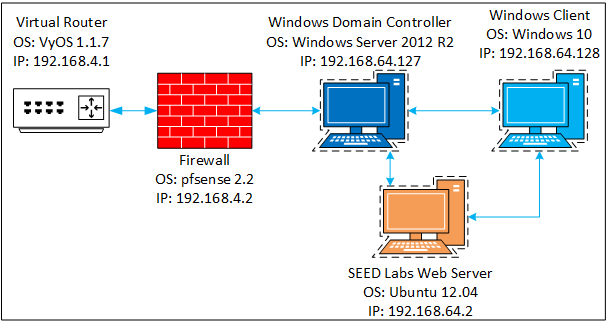
\includegraphics[scale=0.80]{NetworkDiagram.png}
		\end{center}

	\end{instructionblock}
\end{slide}


%----------------------------------------------------------------------------------------------------%





\pagebreak
\begin{slide}{ Network Firewalls Overview }{ \hyperref[slide 4]{\textless}\hyperref[slide 6]{\textgreater} }
\vskip 5pt
\begin{instructionblock}
\begin{enumerate}
\item What are they?
\begin{enumerate}
\item Hardware and/or software based entities used to protect networks from unauthorized access;
\end{enumerate}
\item What are their features?
\begin{enumerate}
\item Stateful Packet Inspection;
\item Network Address Translation (NAT);
\item Virtual Private Networking (VPN).
\end{enumerate}
\end{enumerate}

\end{instructionblock}
\end{slide}


\vspace{8mm}
\ben

\item \textbf{What are they?}
\begin{enumerate}
\item Network firewalls are usually located at the boundary between the internal network and external networks (Perimeter Firewall) or between internal segments of networks (Interior Firewall).
\end{enumerate}
\item \textbf{What are their features?}
\begin{enumerate}
\item Operating in the network layer the firewall examines a packet's header and footer and determines if the packet belongs to a valid session. Using this information the firewall decides if a packet should be forwarded to the internal network or rejected.\cite{Zen2017PacketInsp}
\item Network Firewalls are able to change the network address of devices on either side of the firewall to hide the true addresses of devices. This can prevent devices on the outside of a network from being able to probe the true addresses of devices on a network.\cite{UnivHOU2016Firewalls}
\item Network firewalls are able to create encrypted connections using VPNs between themselves. If a host on a network needs to communicate with a host on another network the firewall can establish a secure communication channel with the other host through its firewall.
\end{enumerate}

\een


%----------------------------------------------------------------------------------------------------%





\pagebreak
\begin{slide}{ Types of Network Firewalls }{ \hyperref[slide 5]{\textless}\hyperref[slide 7]{\textgreater} }
\vskip 5pt
\begin{instructionblock}
There are many types of Network Firewalls including: 
\begin{enumerate}
\item Fortinet FortiGate;
\item Cisco ASA;
\item SonicWALL TZ;
\item Cyberoam UTM;
\item pfSense.
\end{enumerate}
We are going to focus on pfSense for this tutorial.
\end{instructionblock}
\end{slide}



%----------------------------------------------------------------------------------------------------%




\pagebreak
\begin{slide}{ In the News }{ \hyperref[slide 6]{\textless}\hyperref[slide 8]{\textgreater} }
\begin{instructionblock}
	\begin{enumerate}
		\item Cisco's ASA firewalls compromised using malformed UDP packets. (11th Feb. 2016) \cite{Cisco2016Constantin} [PCWorld].
		\item Cisco zero day leaked by Shadow Brokers.
		\item Firestorm vulnerability permits extraction of data via TCP handshakes regardless of rules or IP address filters.
	\end{enumerate}
\end{instructionblock}
\end{slide}

\vspace{8mm}
\ben

\item { \textbf{Cisco's ASA Bypass:} Cisco Systems' Adaptive Security Alliance (ASA) firewalls were confronted (and subsequently patched) with a critical bypass vulnerability which had the potential to allow remote attackers to over the firewalls, which are configured as virtual private network servers by simply sending malformed UDP (User Datagram Protocol) network packets to the firewalls \cite{Cisco2016Constantin}.}

\item The Shadow Brokers group released Cisco zero-day  vulnerability. Referred to as EXTRABACON (CVE-2016-6366) deals with the way the firewall handles SNMP protocol. This vulnerability allows attackers to remotely case the system to reload or execute arbitrary code.\cite{Kovacs2016EXTRABACON} Mitigation's for this attack are allowing only trusted users to have SNMP access.

\item Researchers at BugSec Group and Cynet discovered a vulnerability in newer firewalls that allows internal data to be extracted using the handshake of the TCP protocol. The firewalls permit any handshake from an outside entity in order to gather enough data to identify the application being used. An internal actor can then utilize specially crafted TCP handshakes to send data to an awaiting external server, effectively bypassing the firewall. Vendors responded that the vulnerability is by design, and must be allowed in order to gather enough information. \cite{FireStorm-Cynet}
\een


%----------------------------------------------------------------------------------------------------%





\pagebreak
\begin{slide}{ Activity: Design a Network }{ \hyperref[slide 7]{\textless}\hyperref[slide 9]{\textgreater} }
\vskip 5pt
\begin{instructionblock}
 For the computers and their roles given below, create a mapping of the network segments and locations of connected computers.
\begin{itemize}
\item Home network:
    \begin{itemize}
        \item Ubuntu 16.04: user at home connecting across the internet;
        \item Netgear: home router and firewall.
    \end{itemize}
\item Business domain:
    \begin{itemize}
        \item pfSense: domain router and firewall;
        \item Windows Server: domain controller and DNS Server;
        \item Windows 10: employee workstation on the domain;
        \item SEED: web server, for internal and external websites.
    \end{itemize}
\item VyOS router: acting as ``the internet".
\end{itemize}
\end{instructionblock}
\end{slide}


\vspace{8mm}
\ben
    \item The design should express the appropriate segmentation necessary to separate and protect the concerns of each network of users.
    \item For VyOS, consider it to have 2 interfaces: the connection to the home network, and the connection to the business network. Think of it as the ISP for the home network and simultaneously the ISP for the business network.
    \item For pfSense, consider it to have at least 3 interfaces: WAN, LAN, and DMZ. Does it need more?
    \item Where should firewalls be placed on a given network segment?
    \item For the business domain, how do you separate computers that interact with both internal and external users?
\een



%----------------------------------------------------------------------------------------------------%





\pagebreak
\begin{slide}{ Activity: Set up pfSense }{ \hyperref[slide 8]{\textless}\hyperref[slide 10]{\textgreater} }
\vskip 5pt
\begin{instructionblock}
\begin{enumerate}
\item Deploy pfSense for the "business" domain.
\begin{itemize}
    \item Configure the three interfaces of pfSense:
    \begin{enumerate}
        \item WAN;
        \item LAN;
        \item DMZ (OPT1).
    \end{enumerate}
    
\end{itemize}
\end{enumerate}
\end{instructionblock}
\end{slide}


\vspace{8mm}
\begin{enumerate}
\item Open a console to the pfSense VM.
\item At the menu, notice that initially \texttt{WAN} and \texttt{LAN} are the only network interfaces listed.

\item Enter \textbf{1} for ``{\texttt{Assign interfaces}}".
\item Enter \textbf{n} to skip creating VLANs.
\item For the \texttt{WAN} interface, enter \textbf{vmx0}.
\item For the \texttt{LAN} interface, enter \textbf{vmx1}.
\item For the \texttt{Optional 1} interface, enter \textbf{vmx2}.
\item Press \textbf{enter}, and \textbf{y} to finish and confirm.

\item At the menu, enter \textbf{2} for ``{\texttt{Set interface(s) IP address}}".
\item Enter \textbf{1} for ``WAN".
\item Enter the IP address \textbf{192.168.4.2} . (Most of the time this would be DHCP, assigned by your ISP.)
\item Enter \textbf{30}, for a subnet mask of 255.255.255.252 to indicate 192.168.4.1-2 as the range of addresses that compose your WAN.
\item Next, enter the address of the upstream gateway for your network, \textbf{192.168.4.1} This will allow pfSense to route traffic out of your network. (Normally, this would be the IP address given to you by your ISP.)
\item Press \textbf{Enter} to skip the IPv6 addresses.
\item Enter \textbf{n} to not configure the DHCP server and \textbf{n} again.

\item At the menu again, enter \textbf{2} for ``\texttt{Set interface(s) IP address}"
\item Enter \textbf{2} for ``\texttt{LAN}"
\item Enter the IP address \textbf{192.168.64.1}
\item Enter \textbf{24}, for a subnet mask of 255.255.255.0 to indicate 192.168.64.1-255 as the range of addresses that compose your LAN.
\item Press \textbf{enter} to skip assigning an upstream gateway and to skip the IPv6 option again, and enter \textbf{n} to deny the DHCP server.
\item You will now be provided with a URL to access the GUI for pfSense that will be used later.

\item Repeat the process for the third interface, \texttt{OPT1}. Assign \textbf{192.168.65.1} for the IP address and \textbf{24} for the subnet mask. Otherwise, configure it the same as the LAN.
\end{enumerate}



%----------------------------------------------------------------------------------------------------%





\pagebreak
\begin{slide}{ Activity: Basic Firewall Rules }{ \hyperref[slide 9]{\textless}\hyperref[slide 11]{\textgreater} }
\vskip 5pt
\begin{instructionblock}
What basic rules should be implemented for our business network? Consider:
\begin{enumerate}
    \item WAN;
    \item LAN;
    \item DMZ.
\end{enumerate}
Consider both incoming and outgoing rules.
\end{instructionblock}
\end{slide}


\vspace{8mm}
\noindent
\textbf{Hint}: What services will need to be allowed for each of these interfaces to be able to do their intended function? What are the common functions of a business? Do you want to allow everything from the inside to go out? Would there be downsides to that?



%----------------------------------------------------------------------------------------------------%





\pagebreak
\begin{slide}{ Activity: Log In to pfSense GUI }{ \hyperref[slide 10]{\textless}\hyperref[slide 12]{\textgreater} }
\vskip 5pt
\begin{instructionblock}
From the Windows 10 VM:
\begin{enumerate}
    \item Open up a web browser;
    \item Navigate to the pfSense interface, \textbf{192.168.4.2};
    \item Log in:\\
    User: \textbf{admin};\\
    Password: \textbf{pfsense};
    \item What's the first thing you should do when setting up a new firewall!?
    \item Browse around the variety of menus and options.
\end{enumerate}
\end{instructionblock}
\end{slide}


\vspace{8mm}
\begin{enumerate}
\item Is it a good idea to change the default password of the built-in admin!?
\item Look through all the menus, but particularly note System \textgreater User Manager, Interfaces, Firewall \textgreater NAT and Firewall \textgreater Rules, VPN, and Status \textgreater System Logs.
\item Note the initial state of the rules for each interface under Firewall \textgreater Rules.
\item For an initial task, rename interface \texttt{OPT1} to \texttt{DMZ}.
\item Now go to Interfaces \textgreater WAN, and disable ``\texttt{Block private networks.}" Normally, you wouldn't want to do this. Why? (Because you don't want to allow requests from the outside world that use IP addresses reserved for local networks. Somebody's confused or up to no good.) In our case, however, we're configuring everything utilizing the 192.168.0.0/16 subnet. Was this necessary? or is it simply an interesting experiment in the power of subnetting?
\end{enumerate}



%----------------------------------------------------------------------------------------------------%





\pagebreak
\begin{slide}{ Activity: Basic Lockdown of the LAN }{ \hyperref[slide 11]{\textless}\hyperref[slide 13]{\textgreater} }
\vskip 5pt
\begin{instructionblock}
    For the LAN:
    \begin{itemize}
        \item Allow ICMP out;
        \item Allow DNS access;
        \item Allow users to browse web pages;
        \item Allow FTP from the LAN subnet to anywhere;
        \item Allow SMTP, POP3, and IMAP from LAN subnet to anywhere.
    \end{itemize}
\end{instructionblock}
\end{slide}


\vspace{8mm}
\noindent



%----------------------------------------------------------------------------------------------------%





\pagebreak
\begin{slide}{ Challenge 1: Configure the DMZ }{ \hyperref[slide 12]{\textless}\hyperref[slide 14]{\textgreater} }
\vskip 5pt
\begin{instructionblock}
	For the DMZ:
	\begin{enumerate}
	  \item Allow ICMP and FTP originating from outside DMZ only;
	  \item Allow access to your web server, i.e. for requests from the Ubuntu home user, and from LAN users (think intranet site).
	\end{enumerate}

	\textbf{\Large{Deliverables:}}
	\ben
		\item ICMP and FTP requests originating from inside the DMZ should not work. ICMP requests and FTP requests directed at DMZ nodes from outside should succeed;
		\item All requests from outside the DMZ for web pages located on the DMZ web server should succeed.
	\een

  \vspace{20mm}
  \begin{center}
  \textbf{\Large{Duration: 20-30 min.} }
  \end{center}

\end{instructionblock}
\end{slide}


\vspace{8mm}
\noindent
\textbf{HINTS:}
\begin{enumerate}
    \item Let the DMZ respond to ICMP and FTP requests from the LAN and the WAN, but don't let ICMP or FTP requests originate from the DMZ.
    \item Start with NAT Port Forwarding.
\end{enumerate}



%----------------------------------------------------------------------------------------------------%





\pagebreak
\begin{slide}{ Challenge 2: Set up VPN }{ \hyperref[slide 13]{\textless}\hyperref[slide 15]{\textgreater} }
	\vskip 5pt
\begin{instructionblock}
	Allow the Ubuntu home user to VPN into the LAN
	\begin{enumerate}
	\item Enable the VPN service using OpenVPN;
	\item Configure users for VPN.
	\end{enumerate}

	\textbf{\Large{Deliverables:}}
	\ben
		\item VPN services should be available for accessing nodes located on the LAN for the user accounts created.
	\een

  \vspace{20mm}
  \begin{center}
  \textbf{\Large{Duration: 60 min.} }
  \end{center}

\end{instructionblock}
\end{slide}  


\vspace{8mm}
\noindent
\textbf{HINTS:}\\
You will be using PPTP VPN, take advantage of pfSense logs.



%----------------------------------------------------------------------------------------------------%





% bibliography on last page
\pagebreak
\begin{slide}{ Conclusion }{ \hyperref[slide 14]{\textless}\hyperref[slide 16]{\textgreater} }
	\begin{instructionblock}
		\begin{enumerate}
			\item There are many types of Network firewalls to choose from. Despite the variety, their core functionality is similar;
			\item Firewalls are easy to install and access, but can be relatively difficult to configure for optimal functionality;
			\item Through these walkthroughs and hands-on activities, we've learned some basic pfSense configuration.
		\end{enumerate}
	\end{instructionblock}
\end{slide}





%----------------------------------------------------------------------------------------------------%





\pagebreak	
\begin{slide}{ Appendix: Solutions and Change Log }{ \hyperref[slide 15]{\textless}}
	\begin{instructionblock}
		\begin{enumerate}
			\item {Solutions to the challenges:}
				\ben
					\item Challenge 1;
					\item Challenge 2.
				\een
			\item {Change Log.}
		\end{enumerate}
	\end{instructionblock}
\end{slide}


\vspace{8mm}
\textbf{Solutions to the Challenges:}

\textbf{Challenge 1:}
\begin{enumerate}
\item Allow ICMP and FTP originating from outside DMZ only:
\begin{enumerate}
    \item Go to \textbf{Firewall} \textgreater \textbf{Rules}, ``DMZ" tab.
    \item Click on a \textbf{+} button to start a new rule.
    \item For the rule's settings:
    \begin{itemize}
        \item Action: \textbf{Pass}
        \item Interface: \textbf{DMZ}
        \item Protocol: \textbf{ICMP}
        \item ICMP type: \textbf{any}
        \item Source: \textbf{DMZ net, ``not" checked}
        \item Destination: \textbf{DMZ net*}
        \item Log packets: \textbf{true}
        \item Description: \textbf{(A descriptive name)}
    \end{itemize}
    
    \textbf{*} ``DMZ net" specifies any address on the DMZ subnet; whereas ``DMZ Address" would specify the DMZ interface of pfSense itself.
    
    \item Save and then apply changes.

    \item Click again on a \textbf{+} button to start another rule.
    \item For the rule's settings:
    \begin{itemize}
        \item Action: \textbf{Pass}
        \item Interface: \textbf{DMZ}
        \item Protocol: \textbf{TCP}
        \item ICMP type: \textbf{any}
        \item Source: \textbf{DMZ net, ``not" checked}
        \item Destination: \textbf{DMZ net}
        \item Destination port range: \textbf{FTP (21)}
        \item Log packets: \textbf{true}
        \item Description: \textbf{(A descriptive name)}
    \end{itemize}
    \item Save and then apply changes.
    \item At the very least, test that the rule for ICMP works for a computer on the LAN and for a home computer connecting through pfSense's WAN; and that SEED is conversely unable to ping anything.
\end{enumerate}

\item Allow access to your web server, i.e. for requests from the Ubuntu home user, and from LAN users (think intranet site).
\begin{enumerate}
    \item Go to \textbf{Firewall} \textgreater \textbf{NAT}, ``Port Forward" tab.
    \item Click on a \textbf{+} button to start a new rule.
    \item For the rule's settings:
    \begin{itemize}
        \item Disable: \textbf{unchecked}
        \item No RDR: \textbf{unchecked}
        \item Interface: \textbf{WAN}
        \item Protocol: \textbf{TCP}
        \item Destination: \textbf{WAN net}
        \item Destination port range: \textbf{HTTP}
        \item Redirect target IP: \textbf{192.168.65.2}
        \item Redirect target port: \textbf{HTTP}
        \item Description: \textbf{(A descriptive name)}
        \item NAT reflection: \textbf{Enable (Pure NAT)*}
        \item Filter rule association: \textbf{Rule NAT \textless Description \textgreater**}
    \end{itemize}
    
    \textbf{*} For Nat reflection, if you want to enable computers on the LAN to access the DMZ, set it to \textbf{Enable (Pure NAT)}. This enables their requests to traverse across interfaces, which is normally not permitted. If you were to wish to block requests from the LAN to the DMZ, set it to \textbf{Disable}.
    
    \textbf{**} This lets pfSense automatically create the corresponding rules that the firewall needs for this to work. Let's make this easy on ourselves!
    
    \item Save and then apply changes.
    
    \item Repeat for HTTPS, creating a new rule with all the above settings except selecting \textbf{HTTPS} for Destination port range instead.
    
    \item Test that a home computer connecting through pfSense's WAN and a computer on the LAN, if enabled, can connect to the default site on the SEED server. To do so, simply use the target's IP address (rather than any website name, to avoid setting up DNS or modifying Hosts files).
    
    But what is the actual target whose IP address you need to send the request to? It's 192.168.4.2, the WAN interface of pfSense itself. Why?
\end{enumerate}

\end{enumerate}

 

\vspace{4mm}
\textbf{Challenge 2:}
\begin{enumerate}
\item Go to \textbf{VPN} \textgreater \textbf{PPTP}.
\item Click ``Enable PPTP server".
\item Enter a \textbf{Server address}, 192.168.64.127
\item Enter a \textbf{Remote address range}, 192.168.64.128
\item Enter the Windows Server address in \textbf{PPTP DNS SERVERS} 1st slot, 192.164.64.2
\item Click ``Require 128-bit encryption"
\item  ``Save" your entries.

\item Navigate to ``Users" tab to create a VPN user.
\item Select the icon to create a new user.
\item Enter the desired ``username" and ``password".
\item Save and then apply changes.

\item Next navigate to \textbf{Firewall} \textgreater \textbf{Rules}.
\item Select the ``PPTP VPN" tab.
\item Select the ``Create a new rule icon".
\item For the rule's settings:
\begin{itemize}
    \item Interface: \textbf{PPTP VPN}
    \item Protocol: \textbf{TCP}
    \item Source: \textbf{any}
    \item Destination: \textbf{LAN net}
    \item Destination port range: \textbf{any}
    \item Log packets: \textbf{true}
    \item Description: \textbf{(A descriptive name)}
\end{itemize}
\item Save and then apply changes.

\item On the Ubuntu Client:
    \begin{enumerate}
        \item Open the Network Settings
        \item Select the \textbf{+} icon in the lower left pane to create a new connection.
        \item Interface should be VPN. \textgreater ``Create".
        \item Select the no longer secure PPTP as the connection type \textgreater ``Create".
        \item Enter the IP address of the pfSense WAN for the gateway, 192.168.4.2
        \item Enter the user name you created in pfSense.
        \item Change IPv4 settings method to ``Automatic(VPN) addresses only".
        \item Select \textbf{Advanced}.
        \item in addition to the current settings select ``Use Point-to-Point encryption (MPPE)".
        \item Select 128-bit security and ``Allow stateful encryption".
        \item Save and attempt to connect.
    \end{enumerate}
\end{enumerate}


 
\pagebreak
\textbf{Change Log:}
\label{changelog}

\vspace{4mm}
{
\begin{tabular}{ |p{1cm}|p{3cm}|p{4cm}|p{7cm}|  }
	\hline
	\texttt{\textbf{Ver.}} & \texttt{\textbf{Date}} & \texttt{\textbf{Authors}} & \texttt{\textbf{Changes}} \\
	\hline
	v1.0 & Mar 03rd 2017 & Gabe Gibler \& Colton Hotchkiss & First draft of tutorial. \\
	\hline
	v1.1 & May 10th 2017 & Gabe Gibler \& Colton Hotchkiss & Changed to CC-ByNCSA license. Made introductory sections consistent among tutorials. Added the network diagram. Added in the news section. \\
	\hline
	v1.2 & May 12th 2017 & Gabe Gibler \& Colton Hotchkiss & Making body styles consistent among tutorials. \\
	\hline
	v1.3 & July 22nd 2017 & Ananth Jillepalli & Standardization (network layout diagram, edits, consistency, TeX markup cleaning, and more). \\
	\hline

\end{tabular}
}


	
%----------------------------------------------------------------------------------------------------%





% bibliography on last page
\pagebreak
% this style of bibliography shows urls
\bibliographystyle{IEEEtranS}
\bibliography{2017-SP-CS-439-Firewalls02-Bibliography}	



\end{document}